\documentclass[12pt]{article}

\usepackage{graphicx} % Needed to insert images into the document
\setkeys{Gin}{width=\linewidth,totalheight=\textheight,keepaspectratio} % Improves figure scaling
\usepackage{tikz}

\usepackage{setspace, geometry, amsmath, textcomp, amssymb, fancyhdr}
\usepackage{changepage}
\usepackage{dsfont}
\usepackage{MnSymbol}%
\usepackage{wasysym}%
\usepackage{sidecap}


\geometry{top=1in, bottom=1in, left=0.75in, right=0.75in}

\usetikzlibrary{decorations.pathreplacing,calc}
\usetikzlibrary{matrix,decorations.pathreplacing}
\newcommand{\la}{$\leftarrow~$}
\newcommand{\tab}{\indent \hspace{1cm}}
\newcommand{\tb}{\indent \hspace{5mm}}
\newcommand{\emb}[1]{\emph{\textbf{#1}}}


\title{\textbf{3D Convex Hulls \& Lifting Maps}}
\author{Ankush Gupta\\\texttt{gupta@berkeley.edu}}
\date{}
\usepackage{graphicx}
\begin{document}
\maketitle

In the dead-week and after finals, I had some free time and hence I thought that it would be fun to implement the convex-hull algorithm for higher dimensions, as it is one of the most important alogrithms. I implemented the algorithm for three-dimensions.\\

I followed the description in the Dutch book and online references. I am representing the subdivision using a DCEL structure\footnote{ I tried using quad-edges but always ran into some bug; I guess I need to think about quad-edges more deeply.}. I am also using the conflict graph to get expected $\mathcal{O}(n\log n)$ time.\\

The algorithm runs pretty fast (but not quite as fast as my delaunay implementation). The following are its run-times on different sizes of randomly generated points; it was ran on my laptop running which has \texttt{Intel® Core™ i3 CPU M 350 @ 2.27GHz} processor and $4$GB RAM.

\begin{center}
\begin{tabular}{l|l|l}
	10k & 100k & 1000k\\\hline
	0.44 s & 6.28 s & 82.97s\\
\end{tabular}\\
\end{center}


\subsection*{Lifting Maps}
I also ran the algorithm on parabolically lifted 2d-points. The convex-hulls indeed look similar to delaunay triangulations! Below are some screenshots. The 3d convex hull was visualized using OpenSceneGraph,

\begin{figure}[ht]
\begin{minipage}[b]{0.5\linewidth}
\centering
\includegraphics[width=\textwidth]{1.png}
\end{minipage}
\hspace{0.1cm}
\begin{minipage}[b]{0.5\linewidth}
\centering
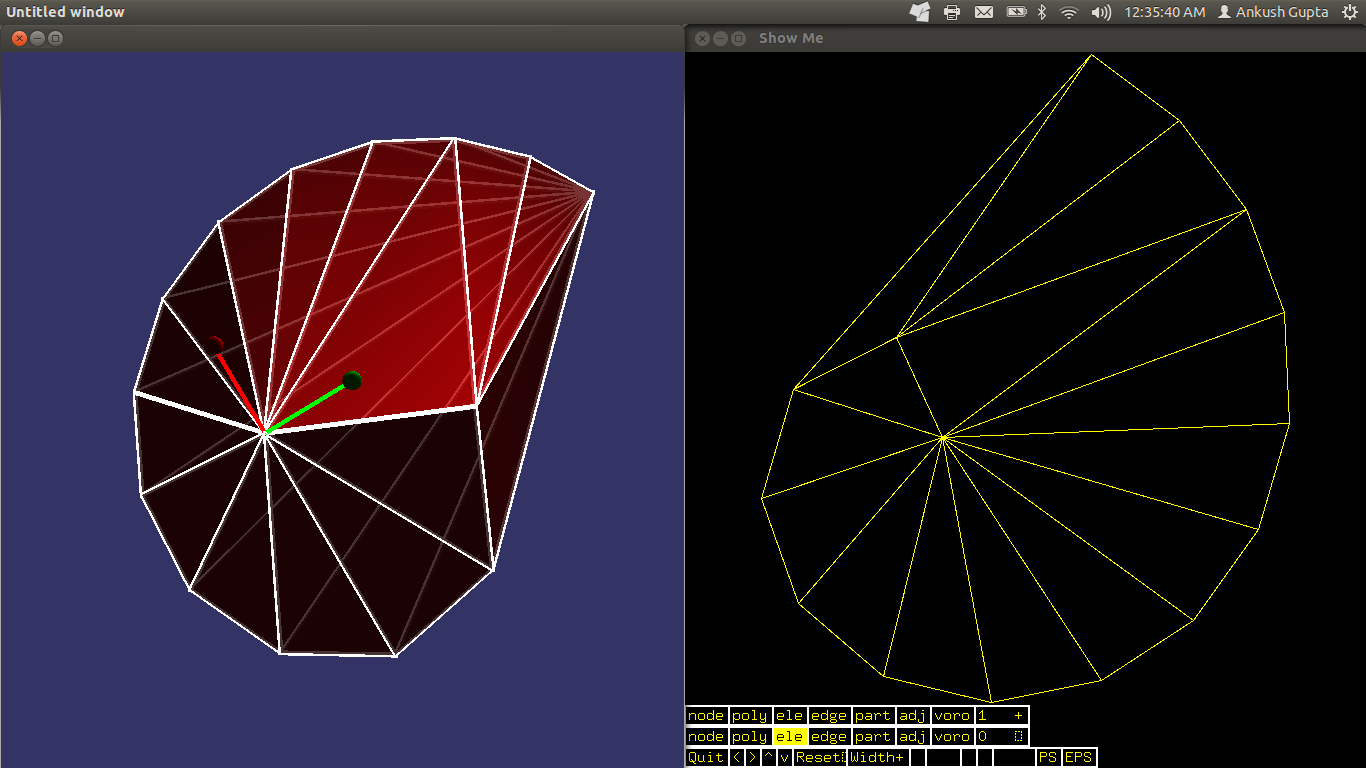
\includegraphics[width=\textwidth]{spiral.png}
\end{minipage}
\caption{Note: The convex-hull (red-colored) has the horizontal axis mirrored, because we are looking from below.}
\end{figure}
\begin{figure}
  \centering
  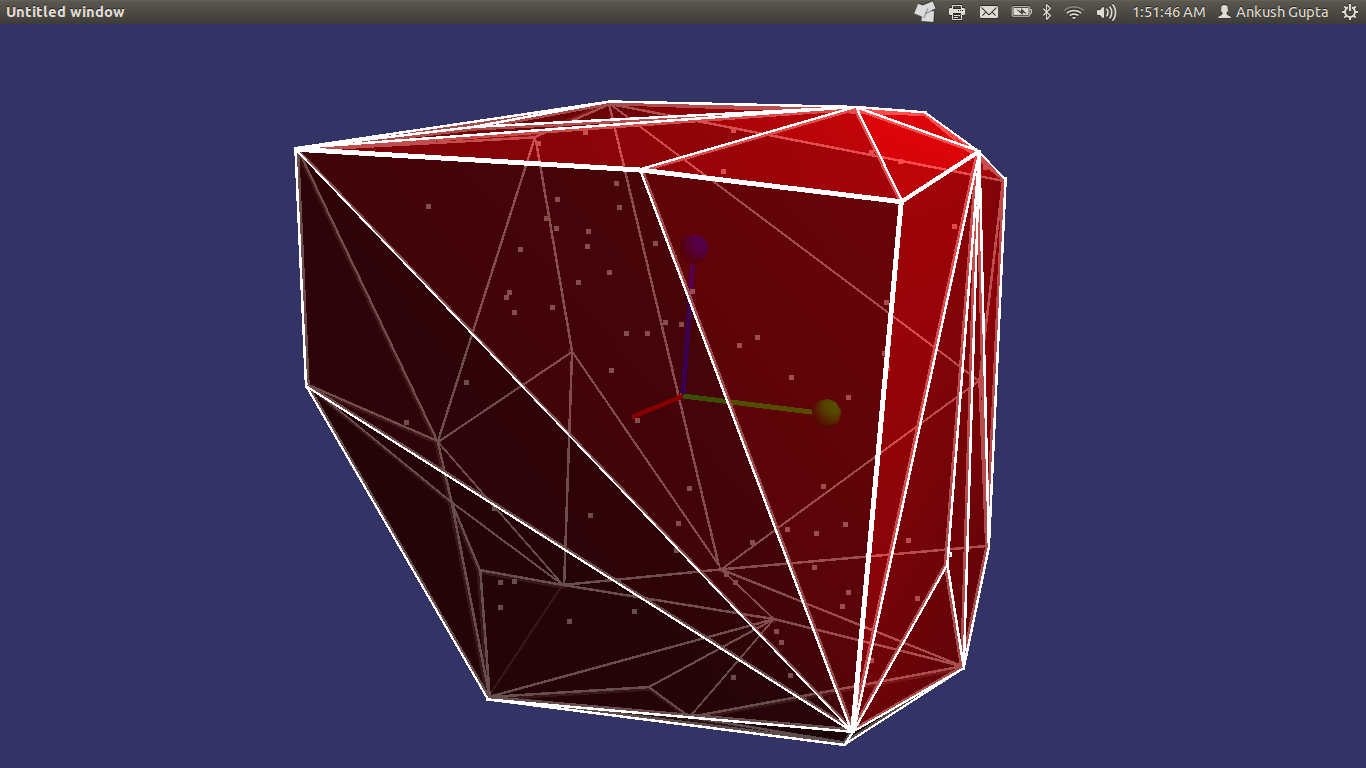
\includegraphics[width=15cm]{rand.png}
  \caption{ Convex hull of some random points.}
\end{figure}

\end{document}